\documentclass[twoside]{book}

% Packages required by doxygen
\usepackage{fixltx2e}
\usepackage{calc}
\usepackage{doxygen}
\usepackage[export]{adjustbox} % also loads graphicx
\usepackage{graphicx}
\usepackage[utf8]{inputenc}
\usepackage{makeidx}
\usepackage{multicol}
\usepackage{multirow}
\PassOptionsToPackage{warn}{textcomp}
\usepackage{textcomp}
\usepackage[nointegrals]{wasysym}
\usepackage[table]{xcolor}

% Font selection
\usepackage[T1]{fontenc}
\usepackage[scaled=.90]{helvet}
\usepackage{courier}
\usepackage{amssymb}
\usepackage{sectsty}
\renewcommand{\familydefault}{\sfdefault}
\allsectionsfont{%
  \fontseries{bc}\selectfont%
  \color{darkgray}%
}
\renewcommand{\DoxyLabelFont}{%
  \fontseries{bc}\selectfont%
  \color{darkgray}%
}
\newcommand{\+}{\discretionary{\mbox{\scriptsize$\hookleftarrow$}}{}{}}

% Page & text layout
\usepackage{geometry}
\geometry{%
  a4paper,%
  top=2.5cm,%
  bottom=2.5cm,%
  left=2.5cm,%
  right=2.5cm%
}
\tolerance=750
\hfuzz=15pt
\hbadness=750
\setlength{\emergencystretch}{15pt}
\setlength{\parindent}{0cm}
\setlength{\parskip}{3ex plus 2ex minus 2ex}
\makeatletter
\renewcommand{\paragraph}{%
  \@startsection{paragraph}{4}{0ex}{-1.0ex}{1.0ex}{%
    \normalfont\normalsize\bfseries\SS@parafont%
  }%
}
\renewcommand{\subparagraph}{%
  \@startsection{subparagraph}{5}{0ex}{-1.0ex}{1.0ex}{%
    \normalfont\normalsize\bfseries\SS@subparafont%
  }%
}
\makeatother

% Headers & footers
\usepackage{fancyhdr}
\pagestyle{fancyplain}
\fancyhead[LE]{\fancyplain{}{\bfseries\thepage}}
\fancyhead[CE]{\fancyplain{}{}}
\fancyhead[RE]{\fancyplain{}{\bfseries\leftmark}}
\fancyhead[LO]{\fancyplain{}{\bfseries\rightmark}}
\fancyhead[CO]{\fancyplain{}{}}
\fancyhead[RO]{\fancyplain{}{\bfseries\thepage}}
\fancyfoot[LE]{\fancyplain{}{}}
\fancyfoot[CE]{\fancyplain{}{}}
\fancyfoot[RE]{\fancyplain{}{\bfseries\scriptsize Generated by Doxygen }}
\fancyfoot[LO]{\fancyplain{}{\bfseries\scriptsize Generated by Doxygen }}
\fancyfoot[CO]{\fancyplain{}{}}
\fancyfoot[RO]{\fancyplain{}{}}
\renewcommand{\footrulewidth}{0.4pt}
\renewcommand{\chaptermark}[1]{%
  \markboth{#1}{}%
}
\renewcommand{\sectionmark}[1]{%
  \markright{\thesection\ #1}%
}

% Indices & bibliography
\usepackage{natbib}
\usepackage[titles]{tocloft}
\setcounter{tocdepth}{3}
\setcounter{secnumdepth}{5}
\makeindex

% Hyperlinks (required, but should be loaded last)
\usepackage{ifpdf}
\ifpdf
  \usepackage[pdftex,pagebackref=true]{hyperref}
\else
  \usepackage[ps2pdf,pagebackref=true]{hyperref}
\fi
\hypersetup{%
  colorlinks=true,%
  linkcolor=blue,%
  citecolor=blue,%
  unicode%
}

% Custom commands
\newcommand{\clearemptydoublepage}{%
  \newpage{\pagestyle{empty}\cleardoublepage}%
}

\usepackage{caption}
\captionsetup{labelsep=space,justification=centering,font={bf},singlelinecheck=off,skip=4pt,position=top}

%===== C O N T E N T S =====

\begin{document}

% Titlepage & ToC
\hypersetup{pageanchor=false,
             bookmarksnumbered=true,
             pdfencoding=unicode
            }
\pagenumbering{alph}
\begin{titlepage}
\vspace*{7cm}
\begin{center}%
{\Large The\+Project }\\
\vspace*{1cm}
{\large Generated by Doxygen 1.8.14}\\
\end{center}
\end{titlepage}
\clearemptydoublepage
\pagenumbering{roman}
\tableofcontents
\clearemptydoublepage
\pagenumbering{arabic}
\hypersetup{pageanchor=true}

%--- Begin generated contents ---
\chapter{The\+Project}
\label{md__c_1_2__i_t__informatik_2__programmierung_1__m_s_v_s2017_entwicklung_1__projekte__the_project69d0b16be0821ba52b290d38ffbeccf6}
\Hypertarget{md__c_1_2__i_t__informatik_2__programmierung_1__m_s_v_s2017_entwicklung_1__projekte__the_project69d0b16be0821ba52b290d38ffbeccf6}
\input{md__c_1_2__i_t__informatik_2__programmierung_1__m_s_v_s2017_entwicklung_1__projekte__the_project69d0b16be0821ba52b290d38ffbeccf6}
\chapter{Bug List}
\label{bug}
\Hypertarget{bug}

\begin{DoxyRefList}
\item[\label{bug__bug000001}%
\Hypertarget{bug__bug000001}%
Member \mbox{\hyperlink{class_input_manager_acf3316661127cbdda5f0bd09cdc46a43}{Input\+Manager\+:\+:Is\+Key\+Down}} (Keyboard\+::\+Key key)]Triggers after a short delay ($\sim$500ms) when placed inside window loop. ~\newline
 
\end{DoxyRefList}
\chapter{Namespace Index}
\section{Namespace List}
Here is a list of all namespaces with brief descriptions\+:\begin{DoxyCompactList}
\item\contentsline{section}{\mbox{\hyperlink{namespace_utils}{Utils}} \\*Contains static functions that serve general purposes }{\pageref{namespace_utils}}{}
\end{DoxyCompactList}

\chapter{Hierarchical Index}
\section{Class Hierarchy}
This inheritance list is sorted roughly, but not completely, alphabetically\+:\begin{DoxyCompactList}
\item \contentsline{section}{Entity}{\pageref{class_entity}}{}
\begin{DoxyCompactList}
\item \contentsline{section}{Drawable\+Entity}{\pageref{class_drawable_entity}}{}
\end{DoxyCompactList}
\item \contentsline{section}{Finite\+State\+Machine}{\pageref{class_finite_state_machine}}{}
\item \contentsline{section}{Input\+Manager}{\pageref{class_input_manager}}{}
\item \contentsline{section}{State}{\pageref{class_state}}{}
\end{DoxyCompactList}

\chapter{Class Index}
\section{Class List}
Here are the classes, structs, unions and interfaces with brief descriptions\+:\begin{DoxyCompactList}
\item\contentsline{section}{\mbox{\hyperlink{class_drawable_entity}{Drawable\+Entity}} }{\pageref{class_drawable_entity}}{}
\item\contentsline{section}{\mbox{\hyperlink{class_entity}{Entity}} }{\pageref{class_entity}}{}
\item\contentsline{section}{\mbox{\hyperlink{class_finite_state_machine}{Finite\+State\+Machine}} }{\pageref{class_finite_state_machine}}{}
\item\contentsline{section}{\mbox{\hyperlink{class_input_manager}{Input\+Manager}} \\*Sollte eher Namespace sein. Klassen nur mit statischen Funktionen sind nicht sinnvoll }{\pageref{class_input_manager}}{}
\item\contentsline{section}{\mbox{\hyperlink{class_state}{State}} }{\pageref{class_state}}{}
\end{DoxyCompactList}

\chapter{File Index}
\section{File List}
Here is a list of all files with brief descriptions\+:\begin{DoxyCompactList}
\item\contentsline{section}{C\+:/2\+\_\+\+I\+T\+\_\+\+Informatik/2\+\_\+\+Programmierung/1\+\_\+\+M\+S\+V\+S2017\+Entwicklung/1\+\_\+\+Projekte/\+The\+Project/\+The\+Project/\+The\+Project/\mbox{\hyperlink{_drawable_entity_8h}{Drawable\+Entity.\+h}} }{\pageref{_drawable_entity_8h}}{}
\item\contentsline{section}{C\+:/2\+\_\+\+I\+T\+\_\+\+Informatik/2\+\_\+\+Programmierung/1\+\_\+\+M\+S\+V\+S2017\+Entwicklung/1\+\_\+\+Projekte/\+The\+Project/\+The\+Project/\+The\+Project/\mbox{\hyperlink{_entity_8h}{Entity.\+h}} }{\pageref{_entity_8h}}{}
\item\contentsline{section}{C\+:/2\+\_\+\+I\+T\+\_\+\+Informatik/2\+\_\+\+Programmierung/1\+\_\+\+M\+S\+V\+S2017\+Entwicklung/1\+\_\+\+Projekte/\+The\+Project/\+The\+Project/\+The\+Project/\mbox{\hyperlink{_finite_state_machine_8cpp}{Finite\+State\+Machine.\+cpp}} }{\pageref{_finite_state_machine_8cpp}}{}
\item\contentsline{section}{C\+:/2\+\_\+\+I\+T\+\_\+\+Informatik/2\+\_\+\+Programmierung/1\+\_\+\+M\+S\+V\+S2017\+Entwicklung/1\+\_\+\+Projekte/\+The\+Project/\+The\+Project/\+The\+Project/\mbox{\hyperlink{_finite_state_machine_8h}{Finite\+State\+Machine.\+h}} }{\pageref{_finite_state_machine_8h}}{}
\item\contentsline{section}{C\+:/2\+\_\+\+I\+T\+\_\+\+Informatik/2\+\_\+\+Programmierung/1\+\_\+\+M\+S\+V\+S2017\+Entwicklung/1\+\_\+\+Projekte/\+The\+Project/\+The\+Project/\+The\+Project/\mbox{\hyperlink{_input_manager_8cpp}{Input\+Manager.\+cpp}} }{\pageref{_input_manager_8cpp}}{}
\item\contentsline{section}{C\+:/2\+\_\+\+I\+T\+\_\+\+Informatik/2\+\_\+\+Programmierung/1\+\_\+\+M\+S\+V\+S2017\+Entwicklung/1\+\_\+\+Projekte/\+The\+Project/\+The\+Project/\+The\+Project/\mbox{\hyperlink{_input_manager_8h}{Input\+Manager.\+h}} }{\pageref{_input_manager_8h}}{}
\item\contentsline{section}{C\+:/2\+\_\+\+I\+T\+\_\+\+Informatik/2\+\_\+\+Programmierung/1\+\_\+\+M\+S\+V\+S2017\+Entwicklung/1\+\_\+\+Projekte/\+The\+Project/\+The\+Project/\+The\+Project/\mbox{\hyperlink{main_8cpp}{main.\+cpp}} }{\pageref{main_8cpp}}{}
\item\contentsline{section}{C\+:/2\+\_\+\+I\+T\+\_\+\+Informatik/2\+\_\+\+Programmierung/1\+\_\+\+M\+S\+V\+S2017\+Entwicklung/1\+\_\+\+Projekte/\+The\+Project/\+The\+Project/\+The\+Project/\mbox{\hyperlink{_state_8cpp}{State.\+cpp}} }{\pageref{_state_8cpp}}{}
\item\contentsline{section}{C\+:/2\+\_\+\+I\+T\+\_\+\+Informatik/2\+\_\+\+Programmierung/1\+\_\+\+M\+S\+V\+S2017\+Entwicklung/1\+\_\+\+Projekte/\+The\+Project/\+The\+Project/\+The\+Project/\mbox{\hyperlink{_state_8h}{State.\+h}} }{\pageref{_state_8h}}{}
\item\contentsline{section}{C\+:/2\+\_\+\+I\+T\+\_\+\+Informatik/2\+\_\+\+Programmierung/1\+\_\+\+M\+S\+V\+S2017\+Entwicklung/1\+\_\+\+Projekte/\+The\+Project/\+The\+Project/\+The\+Project/\mbox{\hyperlink{test_8cpp}{test.\+cpp}} }{\pageref{test_8cpp}}{}
\item\contentsline{section}{C\+:/2\+\_\+\+I\+T\+\_\+\+Informatik/2\+\_\+\+Programmierung/1\+\_\+\+M\+S\+V\+S2017\+Entwicklung/1\+\_\+\+Projekte/\+The\+Project/\+The\+Project/\+The\+Project/\mbox{\hyperlink{_utils_8h}{Utils.\+h}} }{\pageref{_utils_8h}}{}
\end{DoxyCompactList}

\chapter{Namespace Documentation}
\hypertarget{namespace_utils}{}\section{Utils Namespace Reference}
\label{namespace_utils}\index{Utils@{Utils}}


Contains static functions that serve general purposes.  


\subsection*{Functions}
\begin{DoxyCompactItemize}
\item 
void \mbox{\hyperlink{namespace_utils_ac9acd31f817733c17df6460b85553c9b}{Pause\+Console}} ()
\begin{DoxyCompactList}\small\item\em Pauses the Console until Enter/\+Return is pressed. \end{DoxyCompactList}\end{DoxyCompactItemize}


\subsection{Detailed Description}
Contains static functions that serve general purposes. 

\subsection{Function Documentation}
\mbox{\Hypertarget{namespace_utils_ac9acd31f817733c17df6460b85553c9b}\label{namespace_utils_ac9acd31f817733c17df6460b85553c9b}} 
\index{Utils@{Utils}!Pause\+Console@{Pause\+Console}}
\index{Pause\+Console@{Pause\+Console}!Utils@{Utils}}
\subsubsection{\texorpdfstring{Pause\+Console()}{PauseConsole()}}
{\footnotesize\ttfamily void Utils\+::\+Pause\+Console (\begin{DoxyParamCaption}{ }\end{DoxyParamCaption})}



Pauses the Console until Enter/\+Return is pressed. 


\chapter{Class Documentation}
\hypertarget{class_drawable_entity}{}\section{Drawable\+Entity Class Reference}
\label{class_drawable_entity}\index{Drawable\+Entity@{Drawable\+Entity}}


{\ttfamily \#include $<$Drawable\+Entity.\+h$>$}

Inheritance diagram for Drawable\+Entity\+:\begin{figure}[H]
\begin{center}
\leavevmode
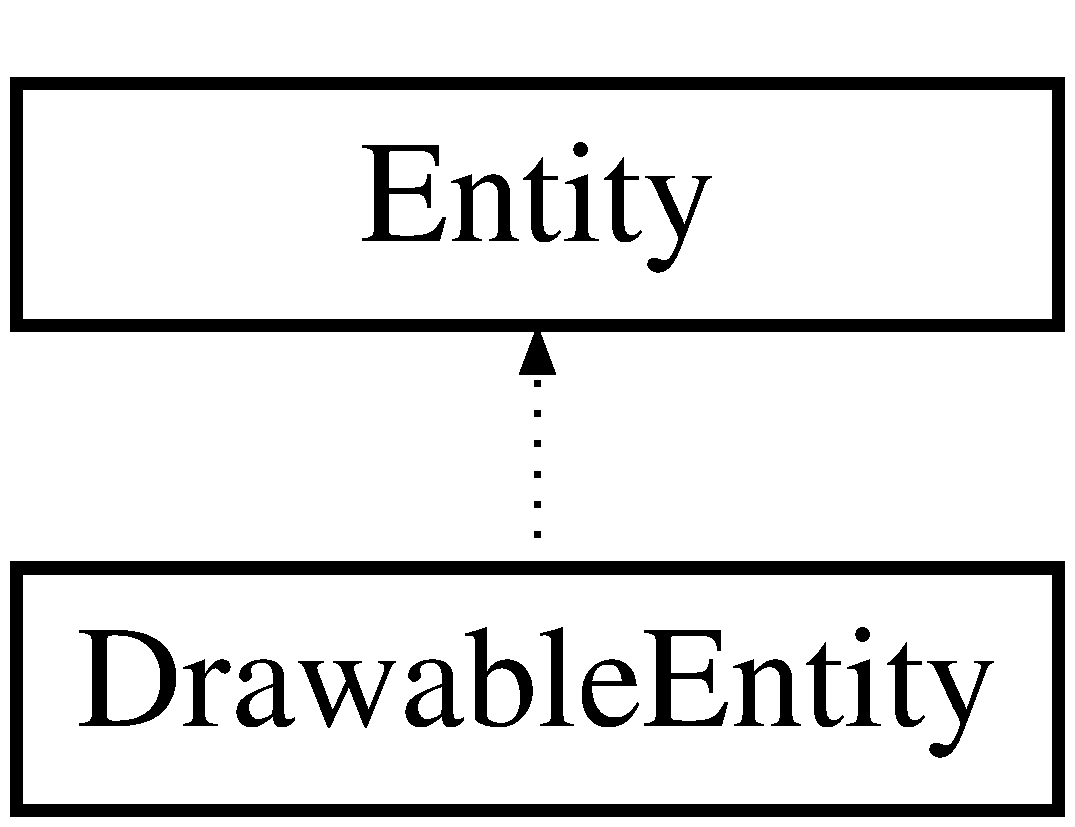
\includegraphics[height=2.000000cm]{class_drawable_entity}
\end{center}
\end{figure}
\subsection*{Public Member Functions}
\begin{DoxyCompactItemize}
\item 
virtual void \mbox{\hyperlink{class_drawable_entity_abc9468e7eb3c1f73eddb9d8b9ae8c93b}{Draw}} ()=0
\end{DoxyCompactItemize}


\subsection{Member Function Documentation}
\mbox{\Hypertarget{class_drawable_entity_abc9468e7eb3c1f73eddb9d8b9ae8c93b}\label{class_drawable_entity_abc9468e7eb3c1f73eddb9d8b9ae8c93b}} 
\index{Drawable\+Entity@{Drawable\+Entity}!Draw@{Draw}}
\index{Draw@{Draw}!Drawable\+Entity@{Drawable\+Entity}}
\subsubsection{\texorpdfstring{Draw()}{Draw()}}
{\footnotesize\ttfamily virtual void Drawable\+Entity\+::\+Draw (\begin{DoxyParamCaption}{ }\end{DoxyParamCaption})\hspace{0.3cm}{\ttfamily [pure virtual]}}



The documentation for this class was generated from the following file\+:\begin{DoxyCompactItemize}
\item 
C\+:/2\+\_\+\+I\+T\+\_\+\+Informatik/2\+\_\+\+Programmierung/1\+\_\+\+M\+S\+V\+S2017\+Entwicklung/1\+\_\+\+Projekte/\+The\+Project/\+The\+Project/\+The\+Project/\mbox{\hyperlink{_drawable_entity_8h}{Drawable\+Entity.\+h}}\end{DoxyCompactItemize}

\hypertarget{class_entity}{}\section{Entity Class Reference}
\label{class_entity}\index{Entity@{Entity}}


{\ttfamily \#include $<$Entity.\+h$>$}

Inheritance diagram for Entity\+:\begin{figure}[H]
\begin{center}
\leavevmode
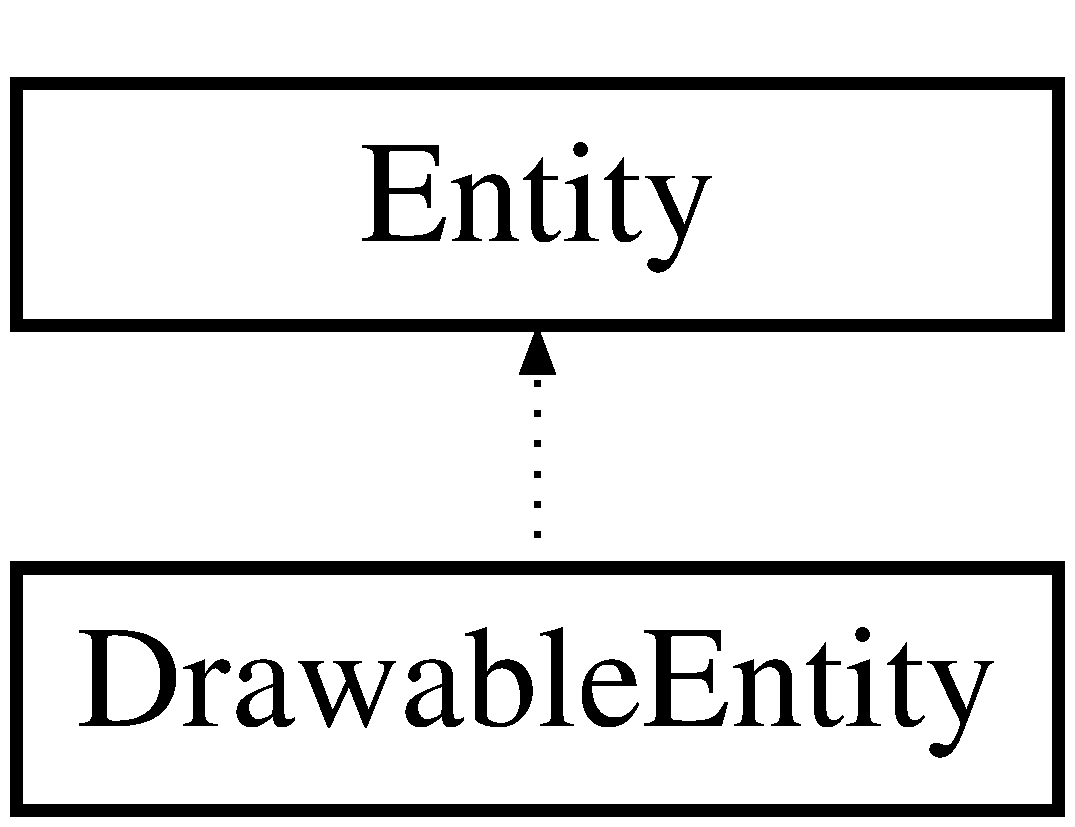
\includegraphics[height=2.000000cm]{class_entity}
\end{center}
\end{figure}
\subsection*{Public Member Functions}
\begin{DoxyCompactItemize}
\item 
virtual void \mbox{\hyperlink{class_entity_a1b842a76a85cd4e4604b253094324b8f}{update}} (float game\+Time)=0
\end{DoxyCompactItemize}


\subsection{Member Function Documentation}
\mbox{\Hypertarget{class_entity_a1b842a76a85cd4e4604b253094324b8f}\label{class_entity_a1b842a76a85cd4e4604b253094324b8f}} 
\index{Entity@{Entity}!update@{update}}
\index{update@{update}!Entity@{Entity}}
\subsubsection{\texorpdfstring{update()}{update()}}
{\footnotesize\ttfamily virtual void Entity\+::update (\begin{DoxyParamCaption}\item[{float}]{game\+Time }\end{DoxyParamCaption})\hspace{0.3cm}{\ttfamily [pure virtual]}}



The documentation for this class was generated from the following file\+:\begin{DoxyCompactItemize}
\item 
C\+:/2\+\_\+\+I\+T\+\_\+\+Informatik/2\+\_\+\+Programmierung/1\+\_\+\+M\+S\+V\+S2017\+Entwicklung/1\+\_\+\+Projekte/\+The\+Project/\+The\+Project/\+The\+Project/\mbox{\hyperlink{_entity_8h}{Entity.\+h}}\end{DoxyCompactItemize}

\hypertarget{class_finite_state_machine}{}\section{Finite\+State\+Machine Class Reference}
\label{class_finite_state_machine}\index{Finite\+State\+Machine@{Finite\+State\+Machine}}


{\ttfamily \#include $<$Finite\+State\+Machine.\+h$>$}

\subsection*{Public Member Functions}
\begin{DoxyCompactItemize}
\item 
\mbox{\hyperlink{class_finite_state_machine_a7f4b2e43939afa064ee2d8232ad9634e}{Finite\+State\+Machine}} ()
\item 
\mbox{\hyperlink{class_finite_state_machine_a841e84d34aa1774e65e6fb4f82ed7635}{Finite\+State\+Machine}} (std\+::map$<$ \mbox{\hyperlink{_finite_state_machine_8h_af5cd382b45a5ef41d63b95e55fbeca95}{E\+State}}, \mbox{\hyperlink{class_state}{State}} $\ast$$>$ $\ast$states, \mbox{\hyperlink{_finite_state_machine_8h_af5cd382b45a5ef41d63b95e55fbeca95}{E\+State}} start\+State, \mbox{\hyperlink{_finite_state_machine_8h_af5cd382b45a5ef41d63b95e55fbeca95}{E\+State}} end\+State)
\item 
\mbox{\hyperlink{class_finite_state_machine_a94fe75c0c063ea1763fd50db3d0199a9}{$\sim$\+Finite\+State\+Machine}} ()
\item 
void \mbox{\hyperlink{class_finite_state_machine_a9b591b86db339b25e188737d813b7a79}{update}} (float game\+Time)
\begin{DoxyCompactList}\small\item\em Updates the current\+State of this \mbox{\hyperlink{class_finite_state_machine}{Finite\+State\+Machine}}. \end{DoxyCompactList}\item 
void \mbox{\hyperlink{class_finite_state_machine_ac5979c2d9ad0adfff26e624d94cf403c}{draw}} ()
\begin{DoxyCompactList}\small\item\em Draws current\+State of this \mbox{\hyperlink{class_finite_state_machine}{Finite\+State\+Machine}}. \end{DoxyCompactList}\item 
bool \mbox{\hyperlink{class_finite_state_machine_a54b47d0d2102026dbb4aa0de9cc4de14}{change}} (\mbox{\hyperlink{_finite_state_machine_8h_af5cd382b45a5ef41d63b95e55fbeca95}{E\+State}} state)
\begin{DoxyCompactList}\small\item\em If possible, changes current\+State of this \mbox{\hyperlink{class_finite_state_machine}{Finite\+State\+Machine}} to state. \end{DoxyCompactList}\item 
void \mbox{\hyperlink{class_finite_state_machine_a04d150c862bab244a86b5ea719d327ad}{reset}} ()
\begin{DoxyCompactList}\small\item\em Resets this \mbox{\hyperlink{class_finite_state_machine}{Finite\+State\+Machine}}(i.\+e. Restores initial \char`\"{}\+State\char`\"{}(colloquial) of this \mbox{\hyperlink{class_finite_state_machine}{Finite\+State\+Machine}}) \end{DoxyCompactList}\item 
void \mbox{\hyperlink{class_finite_state_machine_a8e8f67d3da1a97e45df68d83d356ad8f}{terminate}} ()
\begin{DoxyCompactList}\small\item\em Terminates this \mbox{\hyperlink{class_finite_state_machine}{Finite\+State\+Machine}}(i.\+e. ????) \end{DoxyCompactList}\item 
std\+::map$<$ \mbox{\hyperlink{_finite_state_machine_8h_af5cd382b45a5ef41d63b95e55fbeca95}{E\+State}}, \mbox{\hyperlink{class_state}{State}} $\ast$ $>$ $\ast$ \mbox{\hyperlink{class_finite_state_machine_a432e315a27819cb9a3ed6d6efa4ce563}{get\+States}} ()
\begin{DoxyCompactList}\small\item\em Returns std\+::map with all States of this \mbox{\hyperlink{class_finite_state_machine}{Finite\+State\+Machine}}. \end{DoxyCompactList}\item 
\mbox{\hyperlink{_finite_state_machine_8h_af5cd382b45a5ef41d63b95e55fbeca95}{E\+State}} \mbox{\hyperlink{class_finite_state_machine_afc04978f2883b406a8b9e7141bb31e0e}{get\+Current\+State}} ()
\begin{DoxyCompactList}\small\item\em Returns E\+State current\+State of this \mbox{\hyperlink{class_finite_state_machine}{Finite\+State\+Machine}}. \end{DoxyCompactList}\item 
\mbox{\hyperlink{_finite_state_machine_8h_af5cd382b45a5ef41d63b95e55fbeca95}{E\+State}} \mbox{\hyperlink{class_finite_state_machine_a587822e81306ca1683f8554e6848a82b}{get\+Start\+State}} ()
\begin{DoxyCompactList}\small\item\em Returns E\+State start\+State of this \mbox{\hyperlink{class_finite_state_machine}{Finite\+State\+Machine}}. \end{DoxyCompactList}\item 
\mbox{\hyperlink{_finite_state_machine_8h_af5cd382b45a5ef41d63b95e55fbeca95}{E\+State}} \mbox{\hyperlink{class_finite_state_machine_a23bfa1f48615de9aa17b8ee6f49497f2}{get\+End\+State}} ()
\begin{DoxyCompactList}\small\item\em Returns E\+State end\+State of this \mbox{\hyperlink{class_finite_state_machine}{Finite\+State\+Machine}}. \end{DoxyCompactList}\end{DoxyCompactItemize}


\subsection{Constructor \& Destructor Documentation}
\mbox{\Hypertarget{class_finite_state_machine_a7f4b2e43939afa064ee2d8232ad9634e}\label{class_finite_state_machine_a7f4b2e43939afa064ee2d8232ad9634e}} 
\index{Finite\+State\+Machine@{Finite\+State\+Machine}!Finite\+State\+Machine@{Finite\+State\+Machine}}
\index{Finite\+State\+Machine@{Finite\+State\+Machine}!Finite\+State\+Machine@{Finite\+State\+Machine}}
\subsubsection{\texorpdfstring{Finite\+State\+Machine()}{FiniteStateMachine()}\hspace{0.1cm}{\footnotesize\ttfamily [1/2]}}
{\footnotesize\ttfamily Finite\+State\+Machine\+::\+Finite\+State\+Machine (\begin{DoxyParamCaption}{ }\end{DoxyParamCaption})}

\mbox{\Hypertarget{class_finite_state_machine_a841e84d34aa1774e65e6fb4f82ed7635}\label{class_finite_state_machine_a841e84d34aa1774e65e6fb4f82ed7635}} 
\index{Finite\+State\+Machine@{Finite\+State\+Machine}!Finite\+State\+Machine@{Finite\+State\+Machine}}
\index{Finite\+State\+Machine@{Finite\+State\+Machine}!Finite\+State\+Machine@{Finite\+State\+Machine}}
\subsubsection{\texorpdfstring{Finite\+State\+Machine()}{FiniteStateMachine()}\hspace{0.1cm}{\footnotesize\ttfamily [2/2]}}
{\footnotesize\ttfamily Finite\+State\+Machine\+::\+Finite\+State\+Machine (\begin{DoxyParamCaption}\item[{std\+::map$<$ \mbox{\hyperlink{_finite_state_machine_8h_af5cd382b45a5ef41d63b95e55fbeca95}{E\+State}}, \mbox{\hyperlink{class_state}{State}} $\ast$$>$ $\ast$}]{states,  }\item[{\mbox{\hyperlink{_finite_state_machine_8h_af5cd382b45a5ef41d63b95e55fbeca95}{E\+State}}}]{start\+State,  }\item[{\mbox{\hyperlink{_finite_state_machine_8h_af5cd382b45a5ef41d63b95e55fbeca95}{E\+State}}}]{end\+State }\end{DoxyParamCaption})}

\mbox{\Hypertarget{class_finite_state_machine_a94fe75c0c063ea1763fd50db3d0199a9}\label{class_finite_state_machine_a94fe75c0c063ea1763fd50db3d0199a9}} 
\index{Finite\+State\+Machine@{Finite\+State\+Machine}!````~Finite\+State\+Machine@{$\sim$\+Finite\+State\+Machine}}
\index{````~Finite\+State\+Machine@{$\sim$\+Finite\+State\+Machine}!Finite\+State\+Machine@{Finite\+State\+Machine}}
\subsubsection{\texorpdfstring{$\sim$\+Finite\+State\+Machine()}{~FiniteStateMachine()}}
{\footnotesize\ttfamily Finite\+State\+Machine\+::$\sim$\+Finite\+State\+Machine (\begin{DoxyParamCaption}{ }\end{DoxyParamCaption})}



\subsection{Member Function Documentation}
\mbox{\Hypertarget{class_finite_state_machine_a54b47d0d2102026dbb4aa0de9cc4de14}\label{class_finite_state_machine_a54b47d0d2102026dbb4aa0de9cc4de14}} 
\index{Finite\+State\+Machine@{Finite\+State\+Machine}!change@{change}}
\index{change@{change}!Finite\+State\+Machine@{Finite\+State\+Machine}}
\subsubsection{\texorpdfstring{change()}{change()}}
{\footnotesize\ttfamily bool Finite\+State\+Machine\+::change (\begin{DoxyParamCaption}\item[{\mbox{\hyperlink{_finite_state_machine_8h_af5cd382b45a5ef41d63b95e55fbeca95}{E\+State}}}]{state }\end{DoxyParamCaption})}



If possible, changes current\+State of this \mbox{\hyperlink{class_finite_state_machine}{Finite\+State\+Machine}} to state. 


\begin{DoxyParams}{Parameters}
{\em state} & \mbox{\hyperlink{class_state}{State}} that will be current\+State if \mbox{\hyperlink{class_finite_state_machine_a54b47d0d2102026dbb4aa0de9cc4de14}{change()}} is successful \\
\hline
\end{DoxyParams}
\begin{DoxyReturn}{Returns}
True if change to state was successful, else false 
\end{DoxyReturn}
\mbox{\Hypertarget{class_finite_state_machine_ac5979c2d9ad0adfff26e624d94cf403c}\label{class_finite_state_machine_ac5979c2d9ad0adfff26e624d94cf403c}} 
\index{Finite\+State\+Machine@{Finite\+State\+Machine}!draw@{draw}}
\index{draw@{draw}!Finite\+State\+Machine@{Finite\+State\+Machine}}
\subsubsection{\texorpdfstring{draw()}{draw()}}
{\footnotesize\ttfamily void Finite\+State\+Machine\+::draw (\begin{DoxyParamCaption}{ }\end{DoxyParamCaption})}



Draws current\+State of this \mbox{\hyperlink{class_finite_state_machine}{Finite\+State\+Machine}}. 

\mbox{\Hypertarget{class_finite_state_machine_afc04978f2883b406a8b9e7141bb31e0e}\label{class_finite_state_machine_afc04978f2883b406a8b9e7141bb31e0e}} 
\index{Finite\+State\+Machine@{Finite\+State\+Machine}!get\+Current\+State@{get\+Current\+State}}
\index{get\+Current\+State@{get\+Current\+State}!Finite\+State\+Machine@{Finite\+State\+Machine}}
\subsubsection{\texorpdfstring{get\+Current\+State()}{getCurrentState()}}
{\footnotesize\ttfamily \mbox{\hyperlink{_finite_state_machine_8h_af5cd382b45a5ef41d63b95e55fbeca95}{E\+State}} Finite\+State\+Machine\+::get\+Current\+State (\begin{DoxyParamCaption}{ }\end{DoxyParamCaption})}



Returns E\+State current\+State of this \mbox{\hyperlink{class_finite_state_machine}{Finite\+State\+Machine}}. 

\begin{DoxyReturn}{Returns}
E\+State current\+State of this \mbox{\hyperlink{class_finite_state_machine}{Finite\+State\+Machine}} 
\end{DoxyReturn}
\mbox{\Hypertarget{class_finite_state_machine_a23bfa1f48615de9aa17b8ee6f49497f2}\label{class_finite_state_machine_a23bfa1f48615de9aa17b8ee6f49497f2}} 
\index{Finite\+State\+Machine@{Finite\+State\+Machine}!get\+End\+State@{get\+End\+State}}
\index{get\+End\+State@{get\+End\+State}!Finite\+State\+Machine@{Finite\+State\+Machine}}
\subsubsection{\texorpdfstring{get\+End\+State()}{getEndState()}}
{\footnotesize\ttfamily \mbox{\hyperlink{_finite_state_machine_8h_af5cd382b45a5ef41d63b95e55fbeca95}{E\+State}} Finite\+State\+Machine\+::get\+End\+State (\begin{DoxyParamCaption}{ }\end{DoxyParamCaption})}



Returns E\+State end\+State of this \mbox{\hyperlink{class_finite_state_machine}{Finite\+State\+Machine}}. 

\begin{DoxyReturn}{Returns}
E\+State end\+State of this \mbox{\hyperlink{class_finite_state_machine}{Finite\+State\+Machine}} 
\end{DoxyReturn}
\mbox{\Hypertarget{class_finite_state_machine_a587822e81306ca1683f8554e6848a82b}\label{class_finite_state_machine_a587822e81306ca1683f8554e6848a82b}} 
\index{Finite\+State\+Machine@{Finite\+State\+Machine}!get\+Start\+State@{get\+Start\+State}}
\index{get\+Start\+State@{get\+Start\+State}!Finite\+State\+Machine@{Finite\+State\+Machine}}
\subsubsection{\texorpdfstring{get\+Start\+State()}{getStartState()}}
{\footnotesize\ttfamily \mbox{\hyperlink{_finite_state_machine_8h_af5cd382b45a5ef41d63b95e55fbeca95}{E\+State}} Finite\+State\+Machine\+::get\+Start\+State (\begin{DoxyParamCaption}{ }\end{DoxyParamCaption})}



Returns E\+State start\+State of this \mbox{\hyperlink{class_finite_state_machine}{Finite\+State\+Machine}}. 

\begin{DoxyReturn}{Returns}
E\+State start\+State of this \mbox{\hyperlink{class_finite_state_machine}{Finite\+State\+Machine}} 
\end{DoxyReturn}
\mbox{\Hypertarget{class_finite_state_machine_a432e315a27819cb9a3ed6d6efa4ce563}\label{class_finite_state_machine_a432e315a27819cb9a3ed6d6efa4ce563}} 
\index{Finite\+State\+Machine@{Finite\+State\+Machine}!get\+States@{get\+States}}
\index{get\+States@{get\+States}!Finite\+State\+Machine@{Finite\+State\+Machine}}
\subsubsection{\texorpdfstring{get\+States()}{getStates()}}
{\footnotesize\ttfamily std\+::map$<$ \mbox{\hyperlink{_finite_state_machine_8h_af5cd382b45a5ef41d63b95e55fbeca95}{E\+State}}, \mbox{\hyperlink{class_state}{State}} $\ast$ $>$ $\ast$ Finite\+State\+Machine\+::get\+States (\begin{DoxyParamCaption}{ }\end{DoxyParamCaption})}



Returns std\+::map with all States of this \mbox{\hyperlink{class_finite_state_machine}{Finite\+State\+Machine}}. 

\begin{DoxyReturn}{Returns}
std\+::map with all States of this \mbox{\hyperlink{class_finite_state_machine}{Finite\+State\+Machine}} 
\end{DoxyReturn}
\mbox{\Hypertarget{class_finite_state_machine_a04d150c862bab244a86b5ea719d327ad}\label{class_finite_state_machine_a04d150c862bab244a86b5ea719d327ad}} 
\index{Finite\+State\+Machine@{Finite\+State\+Machine}!reset@{reset}}
\index{reset@{reset}!Finite\+State\+Machine@{Finite\+State\+Machine}}
\subsubsection{\texorpdfstring{reset()}{reset()}}
{\footnotesize\ttfamily void Finite\+State\+Machine\+::reset (\begin{DoxyParamCaption}{ }\end{DoxyParamCaption})}



Resets this \mbox{\hyperlink{class_finite_state_machine}{Finite\+State\+Machine}}(i.\+e. Restores initial \char`\"{}\+State\char`\"{}(colloquial) of this \mbox{\hyperlink{class_finite_state_machine}{Finite\+State\+Machine}}) 

\mbox{\Hypertarget{class_finite_state_machine_a8e8f67d3da1a97e45df68d83d356ad8f}\label{class_finite_state_machine_a8e8f67d3da1a97e45df68d83d356ad8f}} 
\index{Finite\+State\+Machine@{Finite\+State\+Machine}!terminate@{terminate}}
\index{terminate@{terminate}!Finite\+State\+Machine@{Finite\+State\+Machine}}
\subsubsection{\texorpdfstring{terminate()}{terminate()}}
{\footnotesize\ttfamily void Finite\+State\+Machine\+::terminate (\begin{DoxyParamCaption}{ }\end{DoxyParamCaption})}



Terminates this \mbox{\hyperlink{class_finite_state_machine}{Finite\+State\+Machine}}(i.\+e. ????) 

\mbox{\Hypertarget{class_finite_state_machine_a9b591b86db339b25e188737d813b7a79}\label{class_finite_state_machine_a9b591b86db339b25e188737d813b7a79}} 
\index{Finite\+State\+Machine@{Finite\+State\+Machine}!update@{update}}
\index{update@{update}!Finite\+State\+Machine@{Finite\+State\+Machine}}
\subsubsection{\texorpdfstring{update()}{update()}}
{\footnotesize\ttfamily void Finite\+State\+Machine\+::update (\begin{DoxyParamCaption}\item[{float}]{game\+Time }\end{DoxyParamCaption})}



Updates the current\+State of this \mbox{\hyperlink{class_finite_state_machine}{Finite\+State\+Machine}}. 


\begin{DoxyParams}{Parameters}
{\em game\+Time} & ???? Besser w�re Game\+Time Klasse mit mehreren Informationen (elapsed, etc.) \\
\hline
\end{DoxyParams}


The documentation for this class was generated from the following files\+:\begin{DoxyCompactItemize}
\item 
C\+:/2\+\_\+\+I\+T\+\_\+\+Informatik/2\+\_\+\+Programmierung/1\+\_\+\+M\+S\+V\+S2017\+Entwicklung/1\+\_\+\+Projekte/\+The\+Project/\+The\+Project/\+The\+Project/\mbox{\hyperlink{_finite_state_machine_8h}{Finite\+State\+Machine.\+h}}\item 
C\+:/2\+\_\+\+I\+T\+\_\+\+Informatik/2\+\_\+\+Programmierung/1\+\_\+\+M\+S\+V\+S2017\+Entwicklung/1\+\_\+\+Projekte/\+The\+Project/\+The\+Project/\+The\+Project/\mbox{\hyperlink{_finite_state_machine_8cpp}{Finite\+State\+Machine.\+cpp}}\end{DoxyCompactItemize}

\hypertarget{class_input_manager}{}\section{Input\+Manager Class Reference}
\label{class_input_manager}\index{Input\+Manager@{Input\+Manager}}


Sollte eher Namespace sein. Klassen nur mit statischen Funktionen sind nicht sinnvoll.  




{\ttfamily \#include $<$Input\+Manager.\+h$>$}

\subsection*{Public Member Functions}
\begin{DoxyCompactItemize}
\item 
\mbox{\hyperlink{class_input_manager_a8be46886da639b26d67181c29dab6d6c}{Input\+Manager}} ()
\begin{DoxyCompactList}\small\item\em Constructor. \end{DoxyCompactList}\item 
\mbox{\hyperlink{class_input_manager_af518290877dd183606709d5852db5491}{$\sim$\+Input\+Manager}} ()
\begin{DoxyCompactList}\small\item\em Destructor. \end{DoxyCompactList}\item 
void \mbox{\hyperlink{class_input_manager_a93883ab3c8f5bee33e66107515acc3e8}{Update\+Current\+States}} ()
\begin{DoxyCompactList}\small\item\em Updates current Key States. Call before you\textquotesingle{}r Key-\/\+Operations. \end{DoxyCompactList}\item 
void \mbox{\hyperlink{class_input_manager_ac965e4ef52a8a7753c106f2bcae64e21}{Update\+Previous\+States}} ()
\begin{DoxyCompactList}\small\item\em Updates previous Key States. Call after you\textquotesingle{}r Key-\/\+Operations. \end{DoxyCompactList}\item 
bool \mbox{\hyperlink{class_input_manager_a426512406d24de8dd5f0fb2241f6ea3c}{On\+Key\+Down}} (Keyboard\+::\+Key key)
\begin{DoxyCompactList}\small\item\em Gets whether or not key was previously not pressed and is now pressed (=Key\+Press that ignores holding) \end{DoxyCompactList}\item 
bool \mbox{\hyperlink{class_input_manager_a1e80afe2aecb16c9a9b45a111b7f83a5}{On\+Double\+Key\+Down}} (Keyboard\+::\+Key key)
\item 
bool \mbox{\hyperlink{class_input_manager_acf3316661127cbdda5f0bd09cdc46a43}{Is\+Key\+Down}} (Keyboard\+::\+Key key)
\begin{DoxyCompactList}\small\item\em Gets whether or not key was previously pressed and is now pressed as well (=Key\+Press with holding) \end{DoxyCompactList}\end{DoxyCompactItemize}


\subsection{Detailed Description}
Sollte eher Namespace sein. Klassen nur mit statischen Funktionen sind nicht sinnvoll. 

\subsection{Constructor \& Destructor Documentation}
\mbox{\Hypertarget{class_input_manager_a8be46886da639b26d67181c29dab6d6c}\label{class_input_manager_a8be46886da639b26d67181c29dab6d6c}} 
\index{Input\+Manager@{Input\+Manager}!Input\+Manager@{Input\+Manager}}
\index{Input\+Manager@{Input\+Manager}!Input\+Manager@{Input\+Manager}}
\subsubsection{\texorpdfstring{Input\+Manager()}{InputManager()}}
{\footnotesize\ttfamily Input\+Manager\+::\+Input\+Manager (\begin{DoxyParamCaption}{ }\end{DoxyParamCaption})}



Constructor. 

\mbox{\Hypertarget{class_input_manager_af518290877dd183606709d5852db5491}\label{class_input_manager_af518290877dd183606709d5852db5491}} 
\index{Input\+Manager@{Input\+Manager}!````~Input\+Manager@{$\sim$\+Input\+Manager}}
\index{````~Input\+Manager@{$\sim$\+Input\+Manager}!Input\+Manager@{Input\+Manager}}
\subsubsection{\texorpdfstring{$\sim$\+Input\+Manager()}{~InputManager()}}
{\footnotesize\ttfamily Input\+Manager\+::$\sim$\+Input\+Manager (\begin{DoxyParamCaption}{ }\end{DoxyParamCaption})}



Destructor. 



\subsection{Member Function Documentation}
\mbox{\Hypertarget{class_input_manager_acf3316661127cbdda5f0bd09cdc46a43}\label{class_input_manager_acf3316661127cbdda5f0bd09cdc46a43}} 
\index{Input\+Manager@{Input\+Manager}!Is\+Key\+Down@{Is\+Key\+Down}}
\index{Is\+Key\+Down@{Is\+Key\+Down}!Input\+Manager@{Input\+Manager}}
\subsubsection{\texorpdfstring{Is\+Key\+Down()}{IsKeyDown()}}
{\footnotesize\ttfamily bool Input\+Manager\+::\+Is\+Key\+Down (\begin{DoxyParamCaption}\item[{Keyboard\+::\+Key}]{key }\end{DoxyParamCaption})}



Gets whether or not key was previously pressed and is now pressed as well (=Key\+Press with holding) 

\begin{DoxyRefDesc}{Bug}
\item[\mbox{\hyperlink{bug__bug000001}{Bug}}]Triggers after a short delay ($\sim$500ms) when placed inside window loop. ~\newline
 \end{DoxyRefDesc}
\mbox{\Hypertarget{class_input_manager_a1e80afe2aecb16c9a9b45a111b7f83a5}\label{class_input_manager_a1e80afe2aecb16c9a9b45a111b7f83a5}} 
\index{Input\+Manager@{Input\+Manager}!On\+Double\+Key\+Down@{On\+Double\+Key\+Down}}
\index{On\+Double\+Key\+Down@{On\+Double\+Key\+Down}!Input\+Manager@{Input\+Manager}}
\subsubsection{\texorpdfstring{On\+Double\+Key\+Down()}{OnDoubleKeyDown()}}
{\footnotesize\ttfamily bool Input\+Manager\+::\+On\+Double\+Key\+Down (\begin{DoxyParamCaption}\item[{Keyboard\+::\+Key}]{key }\end{DoxyParamCaption})}

\mbox{\Hypertarget{class_input_manager_a426512406d24de8dd5f0fb2241f6ea3c}\label{class_input_manager_a426512406d24de8dd5f0fb2241f6ea3c}} 
\index{Input\+Manager@{Input\+Manager}!On\+Key\+Down@{On\+Key\+Down}}
\index{On\+Key\+Down@{On\+Key\+Down}!Input\+Manager@{Input\+Manager}}
\subsubsection{\texorpdfstring{On\+Key\+Down()}{OnKeyDown()}}
{\footnotesize\ttfamily bool Input\+Manager\+::\+On\+Key\+Down (\begin{DoxyParamCaption}\item[{Keyboard\+::\+Key}]{key }\end{DoxyParamCaption})}



Gets whether or not key was previously not pressed and is now pressed (=Key\+Press that ignores holding) 

\mbox{\Hypertarget{class_input_manager_a93883ab3c8f5bee33e66107515acc3e8}\label{class_input_manager_a93883ab3c8f5bee33e66107515acc3e8}} 
\index{Input\+Manager@{Input\+Manager}!Update\+Current\+States@{Update\+Current\+States}}
\index{Update\+Current\+States@{Update\+Current\+States}!Input\+Manager@{Input\+Manager}}
\subsubsection{\texorpdfstring{Update\+Current\+States()}{UpdateCurrentStates()}}
{\footnotesize\ttfamily void Input\+Manager\+::\+Update\+Current\+States (\begin{DoxyParamCaption}{ }\end{DoxyParamCaption})}



Updates current Key States. Call before you\textquotesingle{}r Key-\/\+Operations. 

\mbox{\Hypertarget{class_input_manager_ac965e4ef52a8a7753c106f2bcae64e21}\label{class_input_manager_ac965e4ef52a8a7753c106f2bcae64e21}} 
\index{Input\+Manager@{Input\+Manager}!Update\+Previous\+States@{Update\+Previous\+States}}
\index{Update\+Previous\+States@{Update\+Previous\+States}!Input\+Manager@{Input\+Manager}}
\subsubsection{\texorpdfstring{Update\+Previous\+States()}{UpdatePreviousStates()}}
{\footnotesize\ttfamily void Input\+Manager\+::\+Update\+Previous\+States (\begin{DoxyParamCaption}{ }\end{DoxyParamCaption})}



Updates previous Key States. Call after you\textquotesingle{}r Key-\/\+Operations. 



The documentation for this class was generated from the following files\+:\begin{DoxyCompactItemize}
\item 
C\+:/2\+\_\+\+I\+T\+\_\+\+Informatik/2\+\_\+\+Programmierung/1\+\_\+\+M\+S\+V\+S2017\+Entwicklung/1\+\_\+\+Projekte/\+The\+Project/\+The\+Project/\+The\+Project/\mbox{\hyperlink{_input_manager_8h}{Input\+Manager.\+h}}\item 
C\+:/2\+\_\+\+I\+T\+\_\+\+Informatik/2\+\_\+\+Programmierung/1\+\_\+\+M\+S\+V\+S2017\+Entwicklung/1\+\_\+\+Projekte/\+The\+Project/\+The\+Project/\+The\+Project/\mbox{\hyperlink{_input_manager_8cpp}{Input\+Manager.\+cpp}}\end{DoxyCompactItemize}

\hypertarget{class_state}{}\section{State Class Reference}
\label{class_state}\index{State@{State}}


{\ttfamily \#include $<$State.\+h$>$}

\subsection*{Public Member Functions}
\begin{DoxyCompactItemize}
\item 
\mbox{\hyperlink{class_state_ab91bb1dd5aa6260ab2a456581daf9ec2}{State}} ()
\item 
\mbox{\hyperlink{class_state_a79094488d03d0299758e83eda0ae3372}{State}} (std\+::vector$<$ \mbox{\hyperlink{class_entity}{Entity}} $\ast$$>$ $\ast$entities, std\+::vector$<$ \mbox{\hyperlink{_finite_state_machine_8h_af5cd382b45a5ef41d63b95e55fbeca95}{E\+State}} $>$ $\ast$next)
\item 
\mbox{\hyperlink{class_state_afab438d92b90dc18d194dbd9c9c8bab3}{$\sim$\+State}} ()
\item 
void \mbox{\hyperlink{class_state_adfaddb5aedfeca338af219798b37ff60}{update}} (float game\+Time)
\item 
void \mbox{\hyperlink{class_state_a548bbd450e95030e0582013466d71029}{draw}} ()
\begin{DoxyCompactList}\small\item\em Draws all Drawable\+Entities of this \mbox{\hyperlink{class_state}{State}}. \end{DoxyCompactList}\item 
std\+::vector$<$ \mbox{\hyperlink{class_entity}{Entity}} $\ast$ $>$ $\ast$ \mbox{\hyperlink{class_state_aeb13f8cbb9aaac05ce2f48826ac4080e}{get\+Entities}} ()
\begin{DoxyCompactList}\small\item\em Returns std\+::vector with all Entities of this \mbox{\hyperlink{class_state}{State}}. \end{DoxyCompactList}\item 
std\+::vector$<$ \mbox{\hyperlink{_finite_state_machine_8h_af5cd382b45a5ef41d63b95e55fbeca95}{E\+State}} $>$ $\ast$ \mbox{\hyperlink{class_state_a38819e230878dbaf8ef24014c539fe2c}{get\+Next}} ()
\begin{DoxyCompactList}\small\item\em Returns std\+::vector with E\+State \char`\"{}references\char`\"{} of all States that can be reached by this \mbox{\hyperlink{class_state}{State}}. \end{DoxyCompactList}\end{DoxyCompactItemize}


\subsection{Constructor \& Destructor Documentation}
\mbox{\Hypertarget{class_state_ab91bb1dd5aa6260ab2a456581daf9ec2}\label{class_state_ab91bb1dd5aa6260ab2a456581daf9ec2}} 
\index{State@{State}!State@{State}}
\index{State@{State}!State@{State}}
\subsubsection{\texorpdfstring{State()}{State()}\hspace{0.1cm}{\footnotesize\ttfamily [1/2]}}
{\footnotesize\ttfamily State\+::\+State (\begin{DoxyParamCaption}{ }\end{DoxyParamCaption})}

\mbox{\Hypertarget{class_state_a79094488d03d0299758e83eda0ae3372}\label{class_state_a79094488d03d0299758e83eda0ae3372}} 
\index{State@{State}!State@{State}}
\index{State@{State}!State@{State}}
\subsubsection{\texorpdfstring{State()}{State()}\hspace{0.1cm}{\footnotesize\ttfamily [2/2]}}
{\footnotesize\ttfamily State\+::\+State (\begin{DoxyParamCaption}\item[{std\+::vector$<$ \mbox{\hyperlink{class_entity}{Entity}} $\ast$$>$ $\ast$}]{entities,  }\item[{std\+::vector$<$ \mbox{\hyperlink{_finite_state_machine_8h_af5cd382b45a5ef41d63b95e55fbeca95}{E\+State}} $>$ $\ast$}]{next }\end{DoxyParamCaption})}

\mbox{\Hypertarget{class_state_afab438d92b90dc18d194dbd9c9c8bab3}\label{class_state_afab438d92b90dc18d194dbd9c9c8bab3}} 
\index{State@{State}!````~State@{$\sim$\+State}}
\index{````~State@{$\sim$\+State}!State@{State}}
\subsubsection{\texorpdfstring{$\sim$\+State()}{~State()}}
{\footnotesize\ttfamily State\+::$\sim$\+State (\begin{DoxyParamCaption}{ }\end{DoxyParamCaption})}



\subsection{Member Function Documentation}
\mbox{\Hypertarget{class_state_a548bbd450e95030e0582013466d71029}\label{class_state_a548bbd450e95030e0582013466d71029}} 
\index{State@{State}!draw@{draw}}
\index{draw@{draw}!State@{State}}
\subsubsection{\texorpdfstring{draw()}{draw()}}
{\footnotesize\ttfamily void State\+::draw (\begin{DoxyParamCaption}{ }\end{DoxyParamCaption})}



Draws all Drawable\+Entities of this \mbox{\hyperlink{class_state}{State}}. 

\mbox{\Hypertarget{class_state_aeb13f8cbb9aaac05ce2f48826ac4080e}\label{class_state_aeb13f8cbb9aaac05ce2f48826ac4080e}} 
\index{State@{State}!get\+Entities@{get\+Entities}}
\index{get\+Entities@{get\+Entities}!State@{State}}
\subsubsection{\texorpdfstring{get\+Entities()}{getEntities()}}
{\footnotesize\ttfamily std\+::vector$<$ \mbox{\hyperlink{class_entity}{Entity}} $\ast$ $>$ $\ast$ State\+::get\+Entities (\begin{DoxyParamCaption}{ }\end{DoxyParamCaption})}



Returns std\+::vector with all Entities of this \mbox{\hyperlink{class_state}{State}}. 

\begin{DoxyReturn}{Returns}
std\+::vector wit all Entities of this \mbox{\hyperlink{class_state}{State}} 
\end{DoxyReturn}
\mbox{\Hypertarget{class_state_a38819e230878dbaf8ef24014c539fe2c}\label{class_state_a38819e230878dbaf8ef24014c539fe2c}} 
\index{State@{State}!get\+Next@{get\+Next}}
\index{get\+Next@{get\+Next}!State@{State}}
\subsubsection{\texorpdfstring{get\+Next()}{getNext()}}
{\footnotesize\ttfamily std\+::vector$<$ \mbox{\hyperlink{_finite_state_machine_8h_af5cd382b45a5ef41d63b95e55fbeca95}{E\+State}} $>$ $\ast$ State\+::get\+Next (\begin{DoxyParamCaption}{ }\end{DoxyParamCaption})}



Returns std\+::vector with E\+State \char`\"{}references\char`\"{} of all States that can be reached by this \mbox{\hyperlink{class_state}{State}}. 

\begin{DoxyReturn}{Returns}
std\+::vector with E\+State \char`\"{}references\char`\"{} of all States that can be reached by this \mbox{\hyperlink{class_state}{State}} 
\end{DoxyReturn}
\mbox{\Hypertarget{class_state_adfaddb5aedfeca338af219798b37ff60}\label{class_state_adfaddb5aedfeca338af219798b37ff60}} 
\index{State@{State}!update@{update}}
\index{update@{update}!State@{State}}
\subsubsection{\texorpdfstring{update()}{update()}}
{\footnotesize\ttfamily void State\+::update (\begin{DoxyParamCaption}\item[{float}]{game\+Time }\end{DoxyParamCaption})}


\begin{DoxyParams}{Parameters}
{\em game\+Time} & Again, Game\+Time class with more information would be better (elapsed, etc.) \\
\hline
\end{DoxyParams}


The documentation for this class was generated from the following files\+:\begin{DoxyCompactItemize}
\item 
C\+:/2\+\_\+\+I\+T\+\_\+\+Informatik/2\+\_\+\+Programmierung/1\+\_\+\+M\+S\+V\+S2017\+Entwicklung/1\+\_\+\+Projekte/\+The\+Project/\+The\+Project/\+The\+Project/\mbox{\hyperlink{_state_8h}{State.\+h}}\item 
C\+:/2\+\_\+\+I\+T\+\_\+\+Informatik/2\+\_\+\+Programmierung/1\+\_\+\+M\+S\+V\+S2017\+Entwicklung/1\+\_\+\+Projekte/\+The\+Project/\+The\+Project/\+The\+Project/\mbox{\hyperlink{_state_8cpp}{State.\+cpp}}\end{DoxyCompactItemize}

\chapter{File Documentation}
\hypertarget{_drawable_entity_8h}{}\section{C\+:/2\+\_\+\+I\+T\+\_\+\+Informatik/2\+\_\+\+Programmierung/1\+\_\+\+M\+S\+V\+S2017\+Entwicklung/1\+\_\+\+Projekte/\+The\+Project/\+The\+Project/\+The\+Project/\+Drawable\+Entity.h File Reference}
\label{_drawable_entity_8h}\index{C\+:/2\+\_\+\+I\+T\+\_\+\+Informatik/2\+\_\+\+Programmierung/1\+\_\+\+M\+S\+V\+S2017\+Entwicklung/1\+\_\+\+Projekte/\+The\+Project/\+The\+Project/\+The\+Project/\+Drawable\+Entity.\+h@{C\+:/2\+\_\+\+I\+T\+\_\+\+Informatik/2\+\_\+\+Programmierung/1\+\_\+\+M\+S\+V\+S2017\+Entwicklung/1\+\_\+\+Projekte/\+The\+Project/\+The\+Project/\+The\+Project/\+Drawable\+Entity.\+h}}
{\ttfamily \#include \char`\"{}Entity.\+h\char`\"{}}\newline
{\ttfamily \#include $<$S\+F\+M\+L/\+Graphics/\+Render\+Target.\+hpp$>$}\newline
\subsection*{Classes}
\begin{DoxyCompactItemize}
\item 
class \mbox{\hyperlink{class_the_project_1_1_drawable_entity}{The\+Project\+::\+Drawable\+Entity}}
\end{DoxyCompactItemize}
\subsection*{Namespaces}
\begin{DoxyCompactItemize}
\item 
 \mbox{\hyperlink{namespace_the_project}{The\+Project}}
\end{DoxyCompactItemize}

\hypertarget{_entity_8h}{}\section{C\+:/2\+\_\+\+I\+T\+\_\+\+Informatik/2\+\_\+\+Programmierung/1\+\_\+\+M\+S\+V\+S2017\+Entwicklung/1\+\_\+\+Projekte/\+The\+Project/\+The\+Project/\+The\+Project/\+Entity.h File Reference}
\label{_entity_8h}\index{C\+:/2\+\_\+\+I\+T\+\_\+\+Informatik/2\+\_\+\+Programmierung/1\+\_\+\+M\+S\+V\+S2017\+Entwicklung/1\+\_\+\+Projekte/\+The\+Project/\+The\+Project/\+The\+Project/\+Entity.\+h@{C\+:/2\+\_\+\+I\+T\+\_\+\+Informatik/2\+\_\+\+Programmierung/1\+\_\+\+M\+S\+V\+S2017\+Entwicklung/1\+\_\+\+Projekte/\+The\+Project/\+The\+Project/\+The\+Project/\+Entity.\+h}}
\subsection*{Classes}
\begin{DoxyCompactItemize}
\item 
class \mbox{\hyperlink{class_entity}{Entity}}
\end{DoxyCompactItemize}

\hypertarget{_finite_state_machine_8cpp}{}\section{C\+:/2\+\_\+\+I\+T\+\_\+\+Informatik/2\+\_\+\+Programmierung/1\+\_\+\+M\+S\+V\+S2017\+Entwicklung/1\+\_\+\+Projekte/\+The\+Project/\+The\+Project/\+The\+Project/\+Finite\+State\+Machine.cpp File Reference}
\label{_finite_state_machine_8cpp}\index{C\+:/2\+\_\+\+I\+T\+\_\+\+Informatik/2\+\_\+\+Programmierung/1\+\_\+\+M\+S\+V\+S2017\+Entwicklung/1\+\_\+\+Projekte/\+The\+Project/\+The\+Project/\+The\+Project/\+Finite\+State\+Machine.\+cpp@{C\+:/2\+\_\+\+I\+T\+\_\+\+Informatik/2\+\_\+\+Programmierung/1\+\_\+\+M\+S\+V\+S2017\+Entwicklung/1\+\_\+\+Projekte/\+The\+Project/\+The\+Project/\+The\+Project/\+Finite\+State\+Machine.\+cpp}}
{\ttfamily \#include \char`\"{}Finite\+State\+Machine.\+h\char`\"{}}\newline
{\ttfamily \#include \char`\"{}State.\+h\char`\"{}}\newline
{\ttfamily \#include $<$algorithm$>$}\newline
{\ttfamily \#include $<$iostream$>$}\newline
{\ttfamily \#include $<$string$>$}\newline
\subsection*{Namespaces}
\begin{DoxyCompactItemize}
\item 
 \mbox{\hyperlink{namespace_the_project}{The\+Project}}
\end{DoxyCompactItemize}

\hypertarget{_finite_state_machine_8h}{}\section{C\+:/2\+\_\+\+I\+T\+\_\+\+Informatik/2\+\_\+\+Programmierung/1\+\_\+\+M\+S\+V\+S2017\+Entwicklung/1\+\_\+\+Projekte/\+The\+Project/\+The\+Project/\+The\+Project/\+Finite\+State\+Machine.h File Reference}
\label{_finite_state_machine_8h}\index{C\+:/2\+\_\+\+I\+T\+\_\+\+Informatik/2\+\_\+\+Programmierung/1\+\_\+\+M\+S\+V\+S2017\+Entwicklung/1\+\_\+\+Projekte/\+The\+Project/\+The\+Project/\+The\+Project/\+Finite\+State\+Machine.\+h@{C\+:/2\+\_\+\+I\+T\+\_\+\+Informatik/2\+\_\+\+Programmierung/1\+\_\+\+M\+S\+V\+S2017\+Entwicklung/1\+\_\+\+Projekte/\+The\+Project/\+The\+Project/\+The\+Project/\+Finite\+State\+Machine.\+h}}
{\ttfamily \#include \char`\"{}State.\+h\char`\"{}}\newline
{\ttfamily \#include $<$map$>$}\newline
\subsection*{Classes}
\begin{DoxyCompactItemize}
\item 
class \mbox{\hyperlink{class_finite_state_machine}{Finite\+State\+Machine}}
\end{DoxyCompactItemize}
\subsection*{Enumerations}
\begin{DoxyCompactItemize}
\item 
enum \mbox{\hyperlink{_finite_state_machine_8h_af5cd382b45a5ef41d63b95e55fbeca95}{E\+State}} \{ \mbox{\hyperlink{_finite_state_machine_8h_af5cd382b45a5ef41d63b95e55fbeca95ab7e4e0120a041dbe6528b050c04269e0}{none}}, 
\mbox{\hyperlink{_finite_state_machine_8h_af5cd382b45a5ef41d63b95e55fbeca95a965bb4d35c5fdbea6581f936340a5556}{inventory}}, 
\mbox{\hyperlink{_finite_state_machine_8h_af5cd382b45a5ef41d63b95e55fbeca95a3766dca84536a644e2f680f520e63180}{main\+Menu}}
 \}
\begin{DoxyCompactList}\small\item\em Enum used to quickly access \mbox{\hyperlink{class_state}{State}} objects inside std\+::map states of this \mbox{\hyperlink{class_finite_state_machine}{Finite\+State\+Machine}}. \end{DoxyCompactList}\end{DoxyCompactItemize}


\subsection{Enumeration Type Documentation}
\mbox{\Hypertarget{_finite_state_machine_8h_af5cd382b45a5ef41d63b95e55fbeca95}\label{_finite_state_machine_8h_af5cd382b45a5ef41d63b95e55fbeca95}} 
\index{Finite\+State\+Machine.\+h@{Finite\+State\+Machine.\+h}!E\+State@{E\+State}}
\index{E\+State@{E\+State}!Finite\+State\+Machine.\+h@{Finite\+State\+Machine.\+h}}
\subsubsection{\texorpdfstring{E\+State}{EState}}
{\footnotesize\ttfamily enum \mbox{\hyperlink{_finite_state_machine_8h_af5cd382b45a5ef41d63b95e55fbeca95}{E\+State}}}



Enum used to quickly access \mbox{\hyperlink{class_state}{State}} objects inside std\+::map states of this \mbox{\hyperlink{class_finite_state_machine}{Finite\+State\+Machine}}. 

\begin{DoxyEnumFields}{Enumerator}
\raisebox{\heightof{T}}[0pt][0pt]{\index{none@{none}!Finite\+State\+Machine.\+h@{Finite\+State\+Machine.\+h}}\index{Finite\+State\+Machine.\+h@{Finite\+State\+Machine.\+h}!none@{none}}}\mbox{\Hypertarget{_finite_state_machine_8h_af5cd382b45a5ef41d63b95e55fbeca95ab7e4e0120a041dbe6528b050c04269e0}\label{_finite_state_machine_8h_af5cd382b45a5ef41d63b95e55fbeca95ab7e4e0120a041dbe6528b050c04269e0}} 
none&Represents the absence of a \mbox{\hyperlink{class_state}{State}}. \\
\hline

\raisebox{\heightof{T}}[0pt][0pt]{\index{inventory@{inventory}!Finite\+State\+Machine.\+h@{Finite\+State\+Machine.\+h}}\index{Finite\+State\+Machine.\+h@{Finite\+State\+Machine.\+h}!inventory@{inventory}}}\mbox{\Hypertarget{_finite_state_machine_8h_af5cd382b45a5ef41d63b95e55fbeca95a965bb4d35c5fdbea6581f936340a5556}\label{_finite_state_machine_8h_af5cd382b45a5ef41d63b95e55fbeca95a965bb4d35c5fdbea6581f936340a5556}} 
inventory&Represents the Inventory \mbox{\hyperlink{class_state}{State}}. \\
\hline

\raisebox{\heightof{T}}[0pt][0pt]{\index{main\+Menu@{main\+Menu}!Finite\+State\+Machine.\+h@{Finite\+State\+Machine.\+h}}\index{Finite\+State\+Machine.\+h@{Finite\+State\+Machine.\+h}!main\+Menu@{main\+Menu}}}\mbox{\Hypertarget{_finite_state_machine_8h_af5cd382b45a5ef41d63b95e55fbeca95a3766dca84536a644e2f680f520e63180}\label{_finite_state_machine_8h_af5cd382b45a5ef41d63b95e55fbeca95a3766dca84536a644e2f680f520e63180}} 
main\+Menu&Represents Main\+Menu \mbox{\hyperlink{class_state}{State}}. \\
\hline

\end{DoxyEnumFields}

\hypertarget{_input_manager_8cpp}{}\section{C\+:/2\+\_\+\+I\+T\+\_\+\+Informatik/2\+\_\+\+Programmierung/1\+\_\+\+M\+S\+V\+S2017\+Entwicklung/1\+\_\+\+Projekte/\+The\+Project/\+The\+Project/\+The\+Project/\+Input\+Manager.cpp File Reference}
\label{_input_manager_8cpp}\index{C\+:/2\+\_\+\+I\+T\+\_\+\+Informatik/2\+\_\+\+Programmierung/1\+\_\+\+M\+S\+V\+S2017\+Entwicklung/1\+\_\+\+Projekte/\+The\+Project/\+The\+Project/\+The\+Project/\+Input\+Manager.\+cpp@{C\+:/2\+\_\+\+I\+T\+\_\+\+Informatik/2\+\_\+\+Programmierung/1\+\_\+\+M\+S\+V\+S2017\+Entwicklung/1\+\_\+\+Projekte/\+The\+Project/\+The\+Project/\+The\+Project/\+Input\+Manager.\+cpp}}
{\ttfamily \#include \char`\"{}Input\+Manager.\+h\char`\"{}}\newline
{\ttfamily \#include $<$iostream$>$}\newline
\subsection*{Namespaces}
\begin{DoxyCompactItemize}
\item 
 \mbox{\hyperlink{namespace_the_project}{The\+Project}}
\end{DoxyCompactItemize}

\hypertarget{_input_manager_8h}{}\section{C\+:/2\+\_\+\+I\+T\+\_\+\+Informatik/2\+\_\+\+Programmierung/1\+\_\+\+M\+S\+V\+S2017\+Entwicklung/1\+\_\+\+Projekte/\+The\+Project/\+The\+Project/\+The\+Project/\+Input\+Manager.h File Reference}
\label{_input_manager_8h}\index{C\+:/2\+\_\+\+I\+T\+\_\+\+Informatik/2\+\_\+\+Programmierung/1\+\_\+\+M\+S\+V\+S2017\+Entwicklung/1\+\_\+\+Projekte/\+The\+Project/\+The\+Project/\+The\+Project/\+Input\+Manager.\+h@{C\+:/2\+\_\+\+I\+T\+\_\+\+Informatik/2\+\_\+\+Programmierung/1\+\_\+\+M\+S\+V\+S2017\+Entwicklung/1\+\_\+\+Projekte/\+The\+Project/\+The\+Project/\+The\+Project/\+Input\+Manager.\+h}}
{\ttfamily \#include $<$S\+F\+M\+L/\+Graphics.\+hpp$>$}\newline
{\ttfamily \#include $<$map$>$}\newline
\subsection*{Classes}
\begin{DoxyCompactItemize}
\item 
class \mbox{\hyperlink{class_input_manager}{Input\+Manager}}
\begin{DoxyCompactList}\small\item\em Sollte eher Namespace sein. Klassen nur mit statischen Funktionen sind nicht sinnvoll. \end{DoxyCompactList}\end{DoxyCompactItemize}

\hypertarget{main_8cpp}{}\section{C\+:/2\+\_\+\+I\+T\+\_\+\+Informatik/2\+\_\+\+Programmierung/1\+\_\+\+M\+S\+V\+S2017\+Entwicklung/1\+\_\+\+Projekte/\+The\+Project/\+The\+Project/\+The\+Project/main.cpp File Reference}
\label{main_8cpp}\index{C\+:/2\+\_\+\+I\+T\+\_\+\+Informatik/2\+\_\+\+Programmierung/1\+\_\+\+M\+S\+V\+S2017\+Entwicklung/1\+\_\+\+Projekte/\+The\+Project/\+The\+Project/\+The\+Project/main.\+cpp@{C\+:/2\+\_\+\+I\+T\+\_\+\+Informatik/2\+\_\+\+Programmierung/1\+\_\+\+M\+S\+V\+S2017\+Entwicklung/1\+\_\+\+Projekte/\+The\+Project/\+The\+Project/\+The\+Project/main.\+cpp}}
{\ttfamily \#include $<$iostream$>$}\newline
{\ttfamily \#include $<$string$>$}\newline
{\ttfamily \#include $<$S\+F\+M\+L/\+Graphics.\+hpp$>$}\newline
{\ttfamily \#include \char`\"{}Input\+Manager.\+h\char`\"{}}\newline
\subsection*{Functions}
\begin{DoxyCompactItemize}
\item 
int \mbox{\hyperlink{main_8cpp_ae66f6b31b5ad750f1fe042a706a4e3d4}{main}} ()
\end{DoxyCompactItemize}


\subsection{Function Documentation}
\mbox{\Hypertarget{main_8cpp_ae66f6b31b5ad750f1fe042a706a4e3d4}\label{main_8cpp_ae66f6b31b5ad750f1fe042a706a4e3d4}} 
\index{main.\+cpp@{main.\+cpp}!main@{main}}
\index{main@{main}!main.\+cpp@{main.\+cpp}}
\subsubsection{\texorpdfstring{main()}{main()}}
{\footnotesize\ttfamily int main (\begin{DoxyParamCaption}{ }\end{DoxyParamCaption})}


\hypertarget{_r_e_a_d_m_e_8md}{}\section{C\+:/2\+\_\+\+I\+T\+\_\+\+Informatik/2\+\_\+\+Programmierung/1\+\_\+\+M\+S\+V\+S2017\+Entwicklung/1\+\_\+\+Projekte/\+The\+Project/\+The\+Project/\+The\+Project/\+R\+E\+A\+D\+ME.md File Reference}
\label{_r_e_a_d_m_e_8md}\index{C\+:/2\+\_\+\+I\+T\+\_\+\+Informatik/2\+\_\+\+Programmierung/1\+\_\+\+M\+S\+V\+S2017\+Entwicklung/1\+\_\+\+Projekte/\+The\+Project/\+The\+Project/\+The\+Project/\+R\+E\+A\+D\+M\+E.\+md@{C\+:/2\+\_\+\+I\+T\+\_\+\+Informatik/2\+\_\+\+Programmierung/1\+\_\+\+M\+S\+V\+S2017\+Entwicklung/1\+\_\+\+Projekte/\+The\+Project/\+The\+Project/\+The\+Project/\+R\+E\+A\+D\+M\+E.\+md}}

\hypertarget{_state_8cpp}{}\section{C\+:/2\+\_\+\+I\+T\+\_\+\+Informatik/2\+\_\+\+Programmierung/1\+\_\+\+M\+S\+V\+S2017\+Entwicklung/1\+\_\+\+Projekte/\+The\+Project/\+The\+Project/\+The\+Project/\+State.cpp File Reference}
\label{_state_8cpp}\index{C\+:/2\+\_\+\+I\+T\+\_\+\+Informatik/2\+\_\+\+Programmierung/1\+\_\+\+M\+S\+V\+S2017\+Entwicklung/1\+\_\+\+Projekte/\+The\+Project/\+The\+Project/\+The\+Project/\+State.\+cpp@{C\+:/2\+\_\+\+I\+T\+\_\+\+Informatik/2\+\_\+\+Programmierung/1\+\_\+\+M\+S\+V\+S2017\+Entwicklung/1\+\_\+\+Projekte/\+The\+Project/\+The\+Project/\+The\+Project/\+State.\+cpp}}
{\ttfamily \#include \char`\"{}State.\+h\char`\"{}}\newline
{\ttfamily \#include \char`\"{}Drawable\+Entity.\+h\char`\"{}}\newline

\hypertarget{_state_8h}{}\section{C\+:/2\+\_\+\+I\+T\+\_\+\+Informatik/2\+\_\+\+Programmierung/1\+\_\+\+M\+S\+V\+S2017\+Entwicklung/1\+\_\+\+Projekte/\+The\+Project/\+The\+Project/\+The\+Project/\+State.h File Reference}
\label{_state_8h}\index{C\+:/2\+\_\+\+I\+T\+\_\+\+Informatik/2\+\_\+\+Programmierung/1\+\_\+\+M\+S\+V\+S2017\+Entwicklung/1\+\_\+\+Projekte/\+The\+Project/\+The\+Project/\+The\+Project/\+State.\+h@{C\+:/2\+\_\+\+I\+T\+\_\+\+Informatik/2\+\_\+\+Programmierung/1\+\_\+\+M\+S\+V\+S2017\+Entwicklung/1\+\_\+\+Projekte/\+The\+Project/\+The\+Project/\+The\+Project/\+State.\+h}}
{\ttfamily \#include \char`\"{}Entity.\+h\char`\"{}}\newline
{\ttfamily \#include \char`\"{}Enums.\+h\char`\"{}}\newline
{\ttfamily \#include $<$vector$>$}\newline
\subsection*{Classes}
\begin{DoxyCompactItemize}
\item 
class \mbox{\hyperlink{class_the_project_1_1_state}{The\+Project\+::\+State}}
\begin{DoxyCompactList}\small\item\em K�nnte abstrakt sein. \end{DoxyCompactList}\end{DoxyCompactItemize}
\subsection*{Namespaces}
\begin{DoxyCompactItemize}
\item 
 \mbox{\hyperlink{namespace_the_project}{The\+Project}}
\end{DoxyCompactItemize}

\hypertarget{test_8cpp}{}\section{C\+:/2\+\_\+\+I\+T\+\_\+\+Informatik/2\+\_\+\+Programmierung/1\+\_\+\+M\+S\+V\+S2017\+Entwicklung/1\+\_\+\+Projekte/\+The\+Project/\+The\+Project/\+The\+Project/test.cpp File Reference}
\label{test_8cpp}\index{C\+:/2\+\_\+\+I\+T\+\_\+\+Informatik/2\+\_\+\+Programmierung/1\+\_\+\+M\+S\+V\+S2017\+Entwicklung/1\+\_\+\+Projekte/\+The\+Project/\+The\+Project/\+The\+Project/test.\+cpp@{C\+:/2\+\_\+\+I\+T\+\_\+\+Informatik/2\+\_\+\+Programmierung/1\+\_\+\+M\+S\+V\+S2017\+Entwicklung/1\+\_\+\+Projekte/\+The\+Project/\+The\+Project/\+The\+Project/test.\+cpp}}

\hypertarget{_utils_8h}{}\section{C\+:/2\+\_\+\+I\+T\+\_\+\+Informatik/2\+\_\+\+Programmierung/1\+\_\+\+M\+S\+V\+S2017\+Entwicklung/1\+\_\+\+Projekte/\+The\+Project/\+The\+Project/\+The\+Project/\+Utils.h File Reference}
\label{_utils_8h}\index{C\+:/2\+\_\+\+I\+T\+\_\+\+Informatik/2\+\_\+\+Programmierung/1\+\_\+\+M\+S\+V\+S2017\+Entwicklung/1\+\_\+\+Projekte/\+The\+Project/\+The\+Project/\+The\+Project/\+Utils.\+h@{C\+:/2\+\_\+\+I\+T\+\_\+\+Informatik/2\+\_\+\+Programmierung/1\+\_\+\+M\+S\+V\+S2017\+Entwicklung/1\+\_\+\+Projekte/\+The\+Project/\+The\+Project/\+The\+Project/\+Utils.\+h}}
{\ttfamily \#include $<$iostream$>$}\newline
\subsection*{Namespaces}
\begin{DoxyCompactItemize}
\item 
 \mbox{\hyperlink{namespace_utils}{Utils}}
\begin{DoxyCompactList}\small\item\em Contains static functions that serve general purposes. \end{DoxyCompactList}\end{DoxyCompactItemize}
\subsection*{Functions}
\begin{DoxyCompactItemize}
\item 
void \mbox{\hyperlink{namespace_utils_ac9acd31f817733c17df6460b85553c9b}{Utils\+::\+Pause\+Console}} ()
\begin{DoxyCompactList}\small\item\em Pauses the Console until Enter/\+Return is pressed. \end{DoxyCompactList}\end{DoxyCompactItemize}

%--- End generated contents ---

% Index
\backmatter
\newpage
\phantomsection
\clearemptydoublepage
\addcontentsline{toc}{chapter}{Index}
\printindex

\end{document}
